\documentclass{beamer}
\usepackage[T1]{fontenc}
\usepackage[utf8]{inputenc}
\usepackage{lmodern}
\usepackage{graphicx}			%para imagens
\usepackage{epstopdf} 			%resolve problemas eps-pdf
\usepackage{fancyhdr}			% para o cabeçalho bonito
\usepackage{caption}				%para legendas
\usepackage{placeins} 			%controlar o lugar dos floats
\usepackage{color}
\usepackage{url}
\renewcommand{\UrlFont}{\tiny}
\usepackage{relsize}
\usepackage{hyperref}

\usetheme{Dresden}
\usecolortheme{orchid}
\setbeamertemplate{navigation symbols}{}

\newcommand{\HRule}{\rule{\linewidth}{0.5mm}}

\title{Video Based Mouse Seizure Detection}
\author{Juarez Sampaio}
\titlegraphic{\leavevmode\smash{\raisebox{5.5cm}{\includegraphics[width=0.2\textwidth]{logo}}}}
\institute{Rice University}
\date{\today}


\begin{document}
\begin{frame}
        \titlepage
\end{frame}

\begin{frame}[fragile]
  \frametitle{Content}
  \begin{itemize}
     \item Results of the week
       \begin{itemize}
           \item Sliding window Flow 
           \item Percentage range flow computation
           \item Percentage range sliding window flow computation
           \item Drawing arrows
       \end{itemize}
  \end{itemize}
\end{frame}


\begin{frame}
  \frametitle{The trick is figuring out how to use numpy}
  \begin{itemize}
      \item To average the X frames of shape (h,w) of the sliding window we create a numpy array of shape (X,h,w)
      and then call average on axis 0
      \item The geometry of drawing arrows is quite simple. However, drawing arrows can be time consuming if we do it
        one by one. The trick was computing all the arrows start and end point and then plot them all. Getting the right
        numpy notation was tough.
      \item Most bugs were fixed by using vector.reshape(-1,1) to enforce the dimension I thought I was using.
  \end{itemize}
\end{frame}


\begin{frame}
  \frametitle{Drawing an arrow}
  \begin{figure}
    \centering
    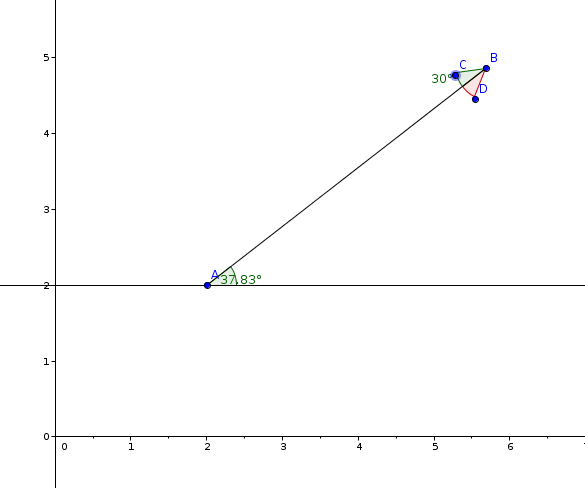
\includegraphics[scale=0.3]{./arrowDraw.png}
    \caption{Find coordinates of points C and D given coordinates A,B and that the arrow angle $\alpha$}
  \end{figure}
\end{frame}

\end{document}
